\documentclass[11pt, letterpaper]{article}

\usepackage[margin=1in]{geometry} % smaller margins
\usepackage{setspace} % set line spacing
\usepackage{hyperref} % Clickable references
\usepackage{appendix} % Appendices
\usepackage{enumitem} % Options for lists
\usepackage{graphicx} % Importing images
\usepackage{amsmath} % Math mode options
\usepackage{cleveref} % Intelligent referencing, with options for hyperlinking and abbreviation
\usepackage{subcaption} % Captions in subfigures
\usepackage{adjustbox}

\setlist[itemize]{noitemsep} % Remove spacing in between items in a list

%
% Define a new command to simplify figures that go into margins
%
\newlength{\overhang}
\setlength{\overhang}{1cm} % Amount the figure will extend into the margin on each side
\newcommand{\fullwidthfigure}[2]{
  \begin{figure}[h]
    \centering
    \makebox[\linewidth]{
      \adjincludegraphics[width=\dimexpr\linewidth+\overhang*2\relax,left=-\overhang]{#1}
    }
    \caption{#2}
  \end{figure}
}

\doublespacing
%\linespread{1.5}

\title{A multiagent model of influence and support in content markets}
\author{Raymond Liu}
\date{November 2023}

\begin{document}

\maketitle

\tableofcontents

\pagebreak

\section{Summary}

The paper \textit{The Role of Social Support and Influencer in Content Markets} takes the idea of a social media community, and breaks in down into two types of agents: community members and influencers. The community members produce content for the community, and consume content created within the community and elsewhere. The influencer serves as an aggregator and distributor within the community, collecting content created within the community and sharing them to everyone. Both community members and consumers can express their interest and support for content items within the community. The paper terms this expression of interest "social support", and proves that it can function as a form of currency. This makes the community a content market in which the agents---content consumers, content producers, and the influencer---act selfishly to produce, consume, or distribute content for their own objectives. The paper also studies the role the influencer plays within this content market: they aggregate content of the most value to the consumers that follow the influencer, and they serve as information proxies to content producers for the amount of social support a content item would receive.

Our work takes this model and implements it computationally as a multiagent system. It simulates the agents and steps through them, each step representing the agent making a decision on who to follow or what topic to produce content on based on the current state of the market. The paper proves that this model will always converge to an equilibrium, and we also find that an equilibrium is reached relatively quickly. We analyze patterns within the resulting followings and content topics within this equilibrium, as they vary depend on specific structural properties within the community. We find that:
\begin{itemize}
    \item Smaller communities tend to be more tight-knit where everyone follow each other, but there is a greater diversity of content topics being produced in larger communities.
    \item When members are more likely to consume content from sources outside the community; they reduce their following to sources inside the community, but they follow the influencer at more-or-less the same rate.
    \item When consumers are generally more interested in a wider range of topics, they are more inclined to follow a greater range of content sources within the community, and they gain more benefit from it.
    \item When producers are generally more capable of producing content on a wider range of topics, they tend to produce content closer to the average interests of the community.
    \item When the influencer has more attention to give to the community, the consumers follow them more, and the influencer plays a greater role in giving value to the community.
    \item When the producers are unable to directly see how much support they receive from the community, and instead must rely on the influencer's following for them as an information proxy: this creates a hierarchy within the community, in which those with interests closer to the average benefit more whereas those with fringe interests seek outside sources.
\end{itemize}

We then compare the social supports and consumer allocations in our model with the ones given within an empirical model of Twitter as a content market, and we attempt to find the set of parameters that match the empirical model most closely. Overall, our model does not closely match with the empirical model, likely due to the amount of randomness and noise. However, we do find some trends, and we conclude that the empirical model of the Twittter community: 
\begin{itemize}
    \item Consumers are broadly interested in many topics within the community, beyond just their main interest.
    \item Whether producers are more or less capable of producing content on topics close to their main interest does not matter significantly.
    \item Influencers and consumers have the same total attention; influencers do not put significantly more attention in the community than consumers.
    \item Producers use the influencer's following as an information proxy on the support they receive, rather than directly optimizing for support from the entire community.
\end{itemize}

\pagebreak

\section{Model}

\subsection{Background}

Given a community in an online social network, the model divides the agents within the community into two broad types. Most agents are \textbf{community members}, who create and produce content, as well as consume and engage with the content created within the community. A select few are \textbf{influencers}, who serve as an aggregators and distributors for the content created by the community members, indicating the popularity and usefulness of the content for the community. For simplicity, the model assumes that there exists only one influencer in each community. This structure of influence is an example of a core-periphery structure in network analysis, as shown in \cref{fig:core-periphery}. The core node (the influencer) serves as a hub or focal point to connect the periphery nodes (the community members) in the network.

\begin{figure}[h]
    \centering
    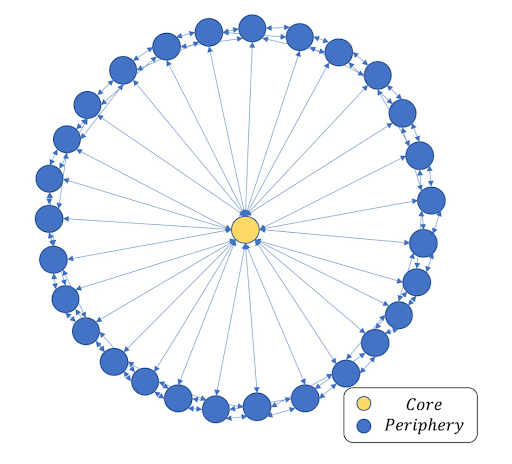
\includegraphics[width=0.4\textwidth]{figures/core-periphery.png}
    \caption{The core-periphery structure}
    \label{fig:core-periphery}
\end{figure}

In order to model this content-creating community as a content market, we also define a mechanism for agents to indicate their interest in the content they consume. We define this as \textbf{social support}, which indicates the level of support given to the content by community members who consume it. In the context of social media, this could be given in the form of likes, shares, comments, and other measures of engagement with the tweet. We can interpret a community member providing social support to a content item as a signal that the content item provides value or utility to them.

With this metric, we can describe the objectives of the agents within the content market. Note that we subdivide community members into content \textbf{consumers} and content \textbf{producers}, since their actions and goals as consumers and producers differ.
\begin{itemize}
    \item Content consumers aim to obtain content that is of interest to them. To do so, they can consume content from other content producers, content shared by the influencer, and from sources from outside the community. We assume that each content consumer has a limited amount of resources or attention to divide between those three types of sources. Consumers indicate their social support (using likes, retweets, etc.) for content items, depending on how much value they receive from it.
    \item Content producers aim to create content that maximize the social support (number of likes, etc.) they receive, by changing the topic on which they produce content.
    \item Influencers aim to attract the most following from content consumers, by sharing content that is of interest to the consumers that follow them. 
\end{itemize}
We assume a game-theoretic model, in which each agent acts selfishly to achieve their own goals, given the information they have on state of the market. The original paper provides the rigorous mathematical structure of this model, formalizing concepts of consumer value, social support, following rates, and so on. We will provide an overview of the mathematical intuition behind this model; for more details, please see the original paper.

\subsection{Mathematical intuition}

Given a community, we assume there is a set of content topics with the notion of a distance between them. For our purposes, we assume the set of topics to be the set of real numbers between \(-1\) and 1, and the distance between topics is represented by how close together the two numbers are. Note that this distance represents how closely two content topics are related; the closer two topics are on the number line, the more related they are.

Then, we assume that each community member (consumer and producer) has a topic which is their main interest. This main interest \(y\) is identified as a real number within the range of \(-1\) to 1. The main interest stays the same throughout the entire model.

Now, set a community member with a main interest \(y\). The probability that they, as a consumer, would be interested in another content topic \(x\) is given by \(f(|x-y|)\), a function of how close together the topic is to the main interest. We assume this function is decreasing, implying that the further apart the topic \(x\) is from the main interest \(y\), the less likely the consumer would be interested in the topic. Similarly, we assume that the ability of the member to produce content in another content topic \(x\) is given by \(g(|x-y|)\), another decreasing function. Therefore, the further apart the topic \(x\) is from the main interest \(y\), the less likely the producer would be able to produce content on that topic.

Each content producer \(y\) produces content on one specific topic, which we represent it as \(x(y)\). Note that this can be different from the content producer's main interest; however, the further away this is from the main interest, the less ability the producer has to produce content on this topic. The content producer changes this value throughout the model, in order to increase the amount of social support that they achieve for the content they produce. 

Each content consumer \(y\) has a maximum amount of attention \(M\) that they can provide to consume content. They divide this attention between the potential sources of content to maximize the value they gain from the content, which are the other content producers, the influencer, and sources outside the community. We assume that they give social support to the content at a rate proportional to the attention they give to the content source. 

The influencer follows and shares content from each content producer at a specific rate, in order to maximize the social support that they have. It has a total rate \(M_\text{INFL}\) that it can divide between all content producers.

\subsubsection{Consumer utility}

We describe in more detail the utility that a content consumer \(y\) obtains from consuming content. The main value of the utility is the probability that a content item created by producer \(z\) is of interest to \(y\). It is calculated as the product of two probabilities: the probability that \(z\) would produce content on the topic it chooses, and the probability that \(y\) would consume content of that topic.

This probability is then scaled by a \textbf{delay}. This is essentially a factor by which the utility is discounted, due to the delay between when a content consumer requests content from a content source, and when the content is received. It is measured as an exponential function involving the rate at which the consumer follows the source; the higher the following rate, the lower the delay and the more utility is obtained by the consumer.

For simplicity, we assume all content producers produce content at the same constant rate, and that sources outside the community produce content at a different constant rate.

With that, the content consumer \(y\)'s utility can be calculated as follows:
\begin{itemize}
    \item Utility from directly following a producer \(z\) and consuming their content: This is the probability that \(z\)'s content is of interest to \(y\), multiplied by the delay and the content production rate.
    \item Utility from viewing a producer \(z\)'s content through the influencer: this is the same probability that \(z\)'s content is of interest to \(y\), with the same content production rate, but multiplied by a different delay. The delay is now the sum of the delay of \(y\) requesting content from the influencer, with the delay of the influencer requesting content from \(z\).
    \item Utility from following sources outside the community: This is based on a constant probability value, representing how likely a content consumer would be interested in a content item produced by an outside source. It is then multiplied by the corresponding delay and production rate.
\end{itemize}
Each utility depends on the following rate that the consumer allocates for it. The total utility is calculated by taking the sum of all the utilities: the utilities of following all the producers directly, following all the producers through the influencer, and outside sources.

\subsubsection{Social support}

As mentioned previously, the social support is the probability in which a content consumer or influencer provides feedback that a content item is of interest to them, such as through likes, retweets, or other forms of engagement. It is the mechanism that influencers and content producers attempt to maximize.

For content consumer \(y\), we assume that the social support \(y\) provides to a content item produced by content producer \(z\) is proportional to the utility that the content item provides to \(y\). This is true for the case where \(y\) follows \(z\) directly, as well as where \(y\) obtain \(z\)'s content through the influencer. 

Thus, when a content producer is maximizing the total social support it receives from all content consumers, it is maximizing the total utility that all content consumers receive from its content directly, as well as through the influencer. 

Similarly, we assume that the social support the influencer provides to a content item produced by content producer \(z\) is proportional to the rate at which the influencer follows \(z\). This means that when \(z\) is maximizing the total social support it receives from all content consumers, it is optimizing the total utility that all content consumers receives from \(z\)'s content, through the influencer. This includes every possible pair of content consumer and producer, except when the content consumer and producer are the same community member.

From this, we can see that when a producer or influencer is optimizing to maximize social support, they are also maximizing the consumer's utilities obtained from the content they produce or share. This means that when a producer or influencer optimizes their allocations to maximize their social support, the total utility over all consumers should only go up as the optimization continues, if all the agents are able to optimize efficiently. We call this total consumer utility the total \textbf{social welfare} of the model, and we can use it as a measure of effectiveness of the model.

\subsection{The optimization problem}

We can now formalize this problem as an optimization problem involving three different classes of agents optimizing their specific values. Each type of agent---producer, consumer, and influencer---optimizes their allocation to maximize a value through the model:
\begin{itemize}
    \item The producers optimize their topic allocation (i.e. the topic they produce content on) to maximize their social support. The topic allocations are bounded to be between \(-1\) and 1.
    \item The consumers optimize their allocation of following rates to all the producers, the influencer, and outside sources to maximize their utilities, constrained by the total allocation maximum \(M\).
    \item The influencer optimizes its allocation of following rates to producers to maximize its social support, constrained by the total allocation maximum \(M_\text{INFL}\).
\end{itemize}

The paper proves the existence of a Nash equilibrium: this means at some point of the optimization, the allocations will converge and the model will reach a final state for all agents. There can be multiple possible equilibria depending on the initial state of the model and the optimization algorithm used. The paper also proves that there exists a equilibria that maximizes the social welfare; however, it does not provide conditions on what conditions are needed to achieve this maximum social welfare.

\subsection{Perfect and limited information}

In order for the agents to effectively optimization their allocations, they must have information on the allocations of all other agents. In particular, for the content producers, they must be able to observe the utilities that all the content consumers obtain from consuming their content. We call this case \textbf{perfect information}, where all agents have access to all the required information.

However, this assumption may not reflective of an actual social network. Particularly in a large community, it is unrealistic to assume that a producer can observe the actions of each and every consumer. More realistically, we consider a \textbf{limited information} model in which the producer uses the influencer's rate allocations as a proxy for the social support they receive.

In this case, the content producer no longer optimizes the topic they produce content on to maximize the social support from all consumers. Instead, they optimize their topic to maximize the social support they receive from the influencer. The paper proves that this case does converge to a Nash equilibrium; however, the optimal equilibrium no longer maximizes the total social welfare like before.

\pagebreak

\section{Multiagent model}

Our multiagent model is created in Python, using the package Mesa. It closely follows the mathematical intuition described in previous sections, with classes representing the three types of agents and their respective optimization functions, with the two different information access cases for the producer. We give each community member a distinct member ID between 0 and [the total number of agents\(-1\)], and this ID is used for both the consumer and producer agents that represent this member.

The model is run until convergence, which is defined as when the producer topic allocations, consumer rate allocations, and influencer rate allocations do not change for a specified number of steps. Once that is achieved, the model is assumed to have reached its equilbrium and returns.

The main interests for the members are set to be evenly spread out between \(-1\) and 1, with member 0 producing content on topic \(-1\) and the member with the largest ID producing content on topic 1. 

Potentially of interest is the scheduler, which is responsible for adding the agents and running their optimization functions in a specific order. Our scheduler alternates between three steps: optimizing all the consumers, optimizing the influencer, and optimizing all the producers. In each step, it optimizes all the agents in a round-robin order. 

\subsection{Parameters}

Our model includes a variety of different parameters. The following list provides the full list and what they are set as by default:
\begin{itemize}
    \item \underline{Optimization method}: the specific mathematical method uses to maximize the utility or social support, as an input to the Python method \texttt{scipy.minimize}. We set it as \texttt{SLSQP}, or sequential least-squares programming; it is a common algorithm that uses a quadratic model to solve nonlinear optimization problems with constraints.
    \item \underline{\(M\) and \(M_\text{INFL}\)}: the total rate budget (i.e. the total amount of attention that can be allocated) for for consumers and influencers. We set it as 5.0 and 10.0 respectively, assuming that influencers have a higher rate budget due to their increased importance in the community.
    \item \underline{The number of members}: the total number of community members, not including the influencer. We set it as 10.
    \item \underline{Information access}: whether the model is perfect information or limited information (i.e. whether the content producers have access to consumer utilities). We set it as the perfect information case. 
    \item \underline{\(B_0\) and \(R_0\)}: the probability that content produced by an outside source is of interest to community members, and the rate of content production of outside sources. We set it as 0.75 and 1.0.
    \item \underline{\(R_P\)}: the rate at which content is produced by content producers. We set it as 1.0.
    \item \underline{\(f\) and \(g\)}: The functions representing how likely a consumer is interested in consuming content on a topic and how able a producer is to produce content on a topic, given the difference between the topic and the main interest of the consumer/producer. Note that this must be decreasing. We set it as a decreasing linear function: \(f(x) = g(x) = 1 - 0.5x\).
    \item \underline{Random initialization}: whether the initial rate and topic allocations are assigned randomly, or deterministically. We set them to be deterministic:
    \begin{itemize}
        \item The initial topic allocations for content producers are set to be their main interest topics, assuming that content producers start off creating content on their main interest.
        \item The initial rate allocations for each content consumer are set to be even across all sources: \(M\) (the total rate budget) divided by [total number of members + 2], with the 2 represent the influencer and outside sources.
        \item The initial rate allocation for the influencer is set to be even across all consumers: \(M_\text{INFL}\) (the total rate budget) divided by the total number of consumers.
    \end{itemize}
    \item \underline{Maximum number of steps}: The maximum number of steps for the model to be run, in case convergence is not reached by then. We set it as 100.
    \item \underline{Convergence steps}: The number of steps that the allocations do not change in order for convergence to be reached. We set it as 10.
\end{itemize}

\section{Results}

\begin{figure}[h]
    \centering
    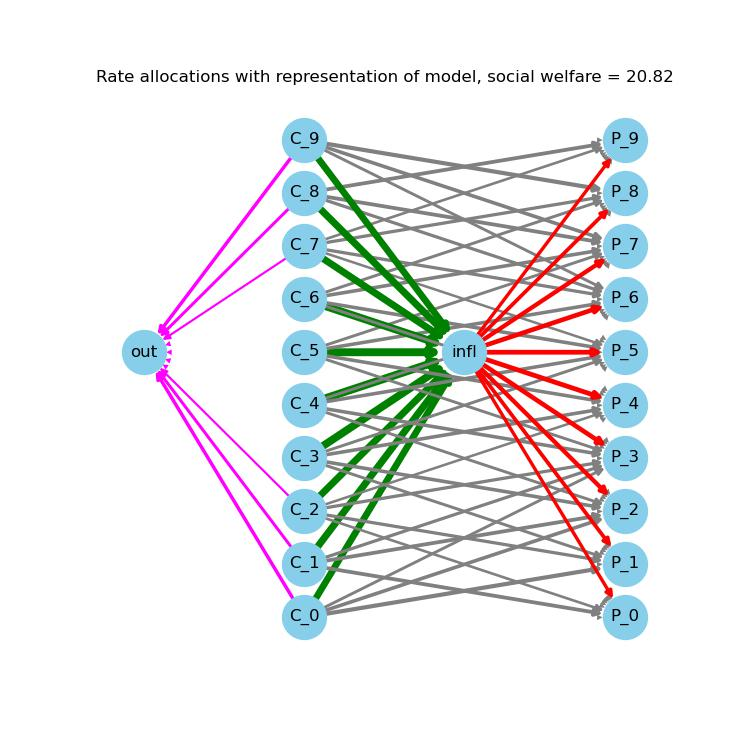
\includegraphics[width=0.65\textwidth]{figures/default_allocs.jpg}
    \caption{Attention flow: Consumer and influencer rate allocations at convergence, given default parameters}
    \label{fig:default_allocs}
\end{figure}

\Cref{fig:default_allocs} shows the rate allocations of the consumer and influencer for the model with default parameters, once convergence is reached in the model. The consumers are lined up in the left column and labelled as C\_[consumer index], whereas the producers are in a corresponding pattern on the right. The "infl" node represents the influencer, and the "out" node represents outside sources.

Each directed edge between nodes represents a non-zero amount of following from a consumer or influencer to a source of content. For the consumers, their rate allocations to the three different types of sources (producers, influencer, outside sources) is represented by three different colors for edges:
\begin{itemize}
    \item The pink edges, from consumers to outside sources, represent the rate allocation of each consumer to the outside sources.
    \item The green edges, from consumers to the influencer, represent the rate allocation of each consumer to the influencer.
    \item The grey edges, from consumer to producer, represent the rate allocation of each consumer to each producer.
\end{itemize}
Finally, the red edges from the influencer to the producers represent the rate allocation of the influencer to the producers.

Note that the width of the edge is proportional to the amount allocated by the agent, and a lack of connections from one agent to another implies that no following is allocated to that agent.

Already, we can see some general trends. The graph is symmetrical, which is expected due to the symmetrical allocation of the members' main interests (evenly spread from \(-1\) to 1). The consumers generally follow producers with main interests close to it. The consumers with main interests closer to the average allocate more following to the influencer, whereas the consumers with main interests further from the average allocate more following to outside sources, as they obtain relatively less value from content shared within the community.

The influencer allocates more attention to producers with main interests closer to the average, because they are more likely to produce content closer to the average main interest, which is of more value to the consumers.

\begin{figure}[h]
    \centering
    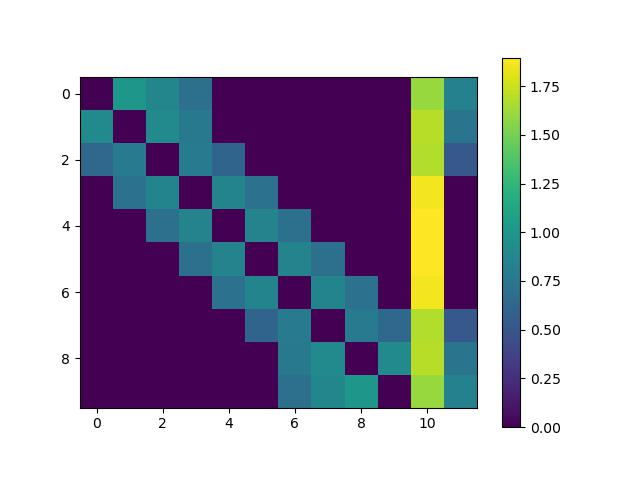
\includegraphics[width=0.6\textwidth]{figures/2D_perfect.jpg}
    \caption{Consumer allocations colormap}
    \label{fig:default_colormap}
\end{figure}

An alternative visualization of the consumer rate allocations is shown in \cref{fig:default_colormap}, where each cell on row \(i\) and column \(j\) represents the allocation that consumer \(i\) provides to producer \(j\), as well as to the influencer (the second column from the right) and outside sources (the rightmost column). It is first evident that the consumer follows the influencer much more than any other source, particularly for the consumers with main interests close to the average. The trends from \cref{fig:default_allocs} can also be confirmed with this figure; consumers tend to follow producers with similar main interests (the blue descending diagonal lines), and consumers closer to the main interest average tend to follow influencers, whereas the consumers further away tend to follow outside sources.

\begin{figure}[h]
    \centering
    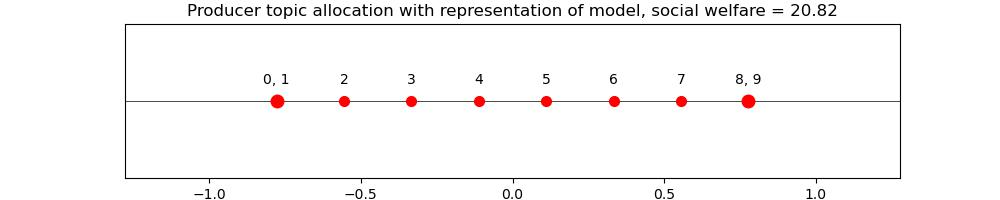
\includegraphics[width=0.8\textwidth]{figures/default_topics.jpg}
    \caption{Producer topic allocations at convergence, given default parameters}
    \label{fig:default_topics}
\end{figure}

The producer topic allocations (the topics that producers create content on) are initially set to be the main interests. \Cref{fig:default_topics} shows the topic allocations once the model reaches convergence; the producers shift their main interests closer to the average, especially the ones that were initially further away.

We will investigate these trends in more detail in following sections by altering parameters away from the default values, and seeing how the resulting rate and topic allocations change.

\subsection{Community size}

\begin{figure}[!h]
    \centering
    \begin{subfigure}[b]{0.2\textwidth}
        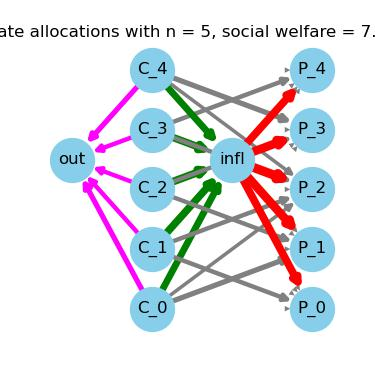
\includegraphics[width=\linewidth]{figures/n/5_allocs.jpg}
    \end{subfigure}
    \begin{subfigure}[b]{0.4\textwidth}
        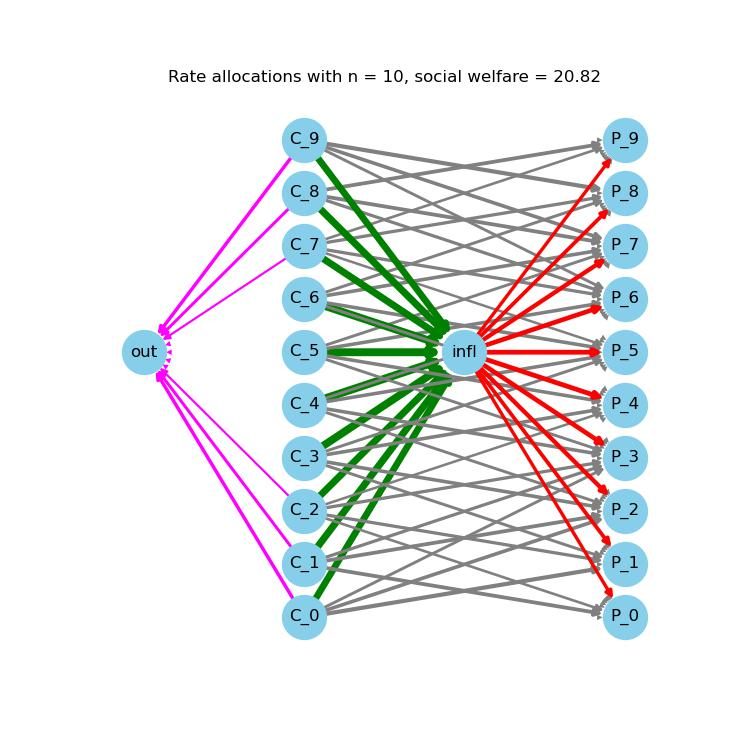
\includegraphics[width=\linewidth]{figures/n/10_allocs.jpg}
    \end{subfigure}
    \begin{subfigure}[b]{0.65\textwidth}
        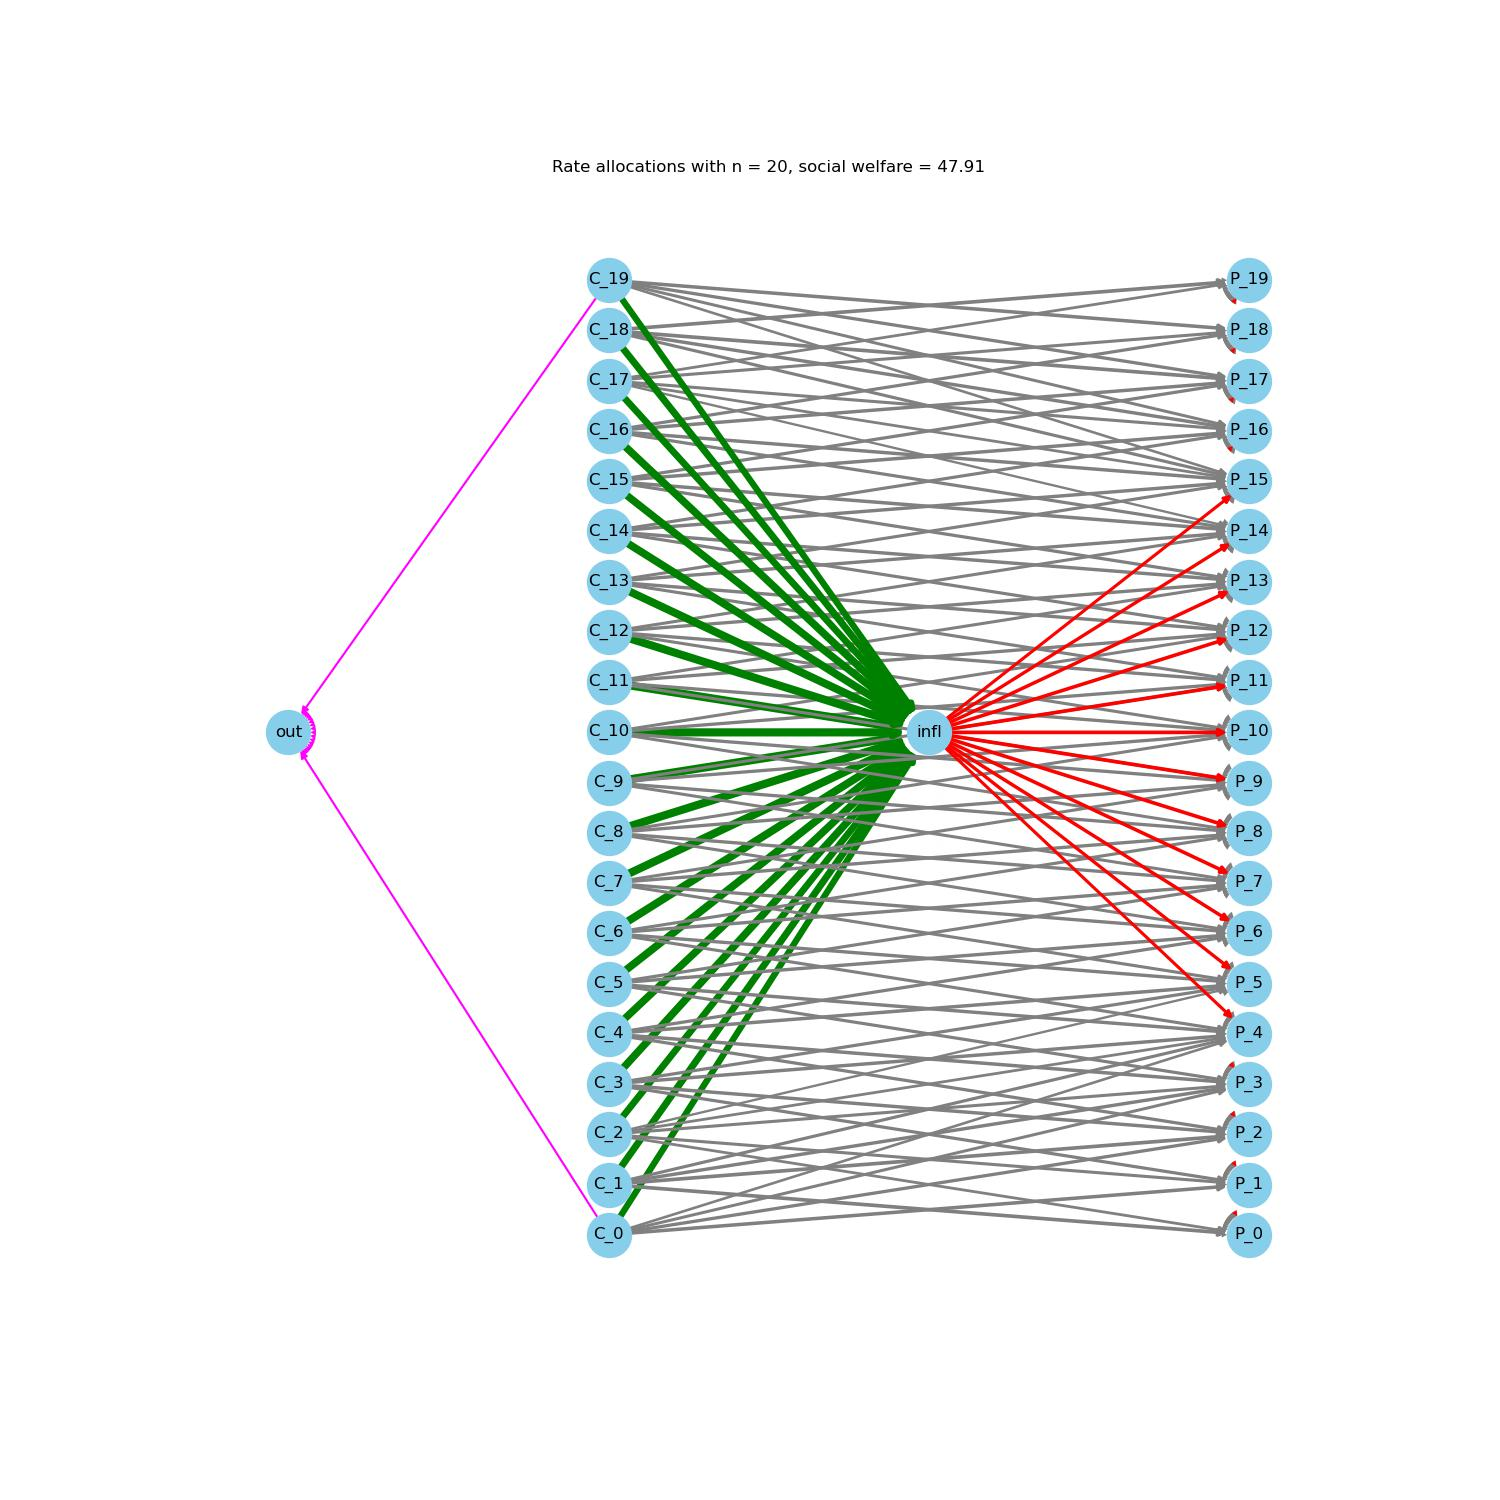
\includegraphics[width=\linewidth]{figures/n/20_allocs.jpg}
    \end{subfigure}
\caption{Rate allocations for different community sizes}
\label{fig:num_members_allocs}
\end{figure}

\Cref{fig:num_members_allocs} shows the rate allocations for the model at different community sizes: 5, 10, and 20. Overall, the smaller the community, the more tightly connected it is. The 5-member community has connections linking nearly every possible pair of agents, with consumers and influencers consuming content from nearly every available source. As the community grows, some consumers stop consuming from outside sources, and they consume content from a lower proportion of producers, specifically those with main interests close to theirs. Similarly, the influencer allocates their rate to a lower proportion of the producers.

However, overall social welfare increases with community size, even when averaging over the number of community members. This suggests that communities with more members foster an increase in the overall benefit provided by the community, simply due to it being larger.

\begin{figure}[h]
    \centering
    \begin{subfigure}[b]{0.6\textwidth}
        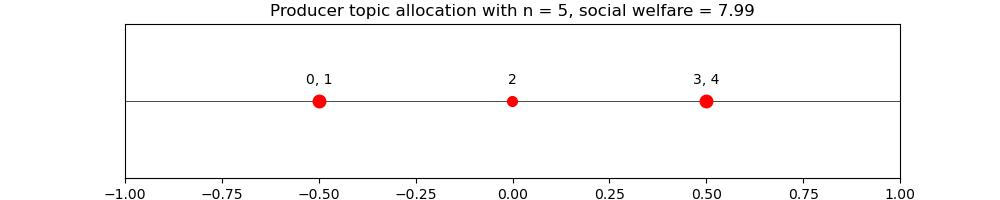
\includegraphics[width=\linewidth]{figures/n/5_topics.jpg}
    \end{subfigure}
    \begin{subfigure}[b]{0.6\textwidth}
        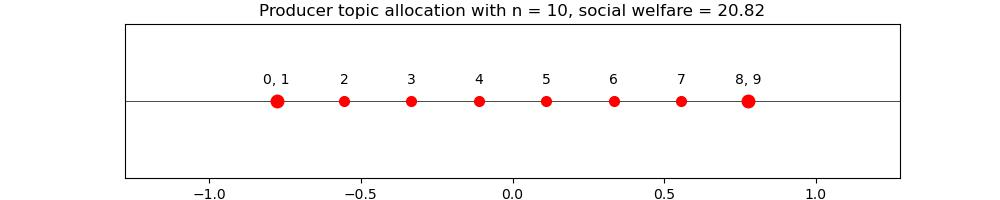
\includegraphics[width=\linewidth]{figures/n/10_topics.jpg}
    \end{subfigure}
    \begin{subfigure}[b]{0.6\textwidth}
        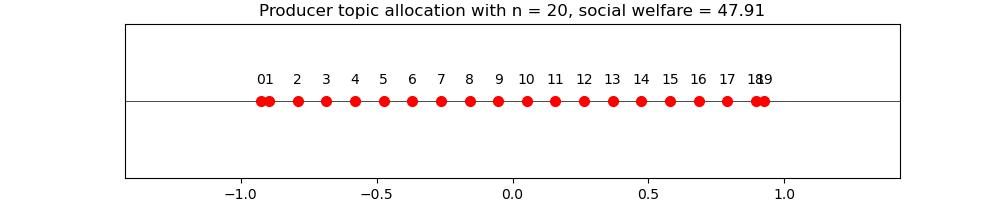
\includegraphics[width=\linewidth]{figures/n/20_topics.jpg}
    \end{subfigure}
\caption{Producer topic allocations for different community sizes}
\label{fig:num_members_topics}
\end{figure}

\Cref{fig:num_members_topics} shows the topic allocations resulting from the different community sizes (which are labelled by the values of \(n\)). Producers from smaller communities produce topics on content much closer to the average, whereas larger communities' topic production remain spread out. Therefore, larger communities encourage a greater diversity in terms of topics produced.

\subsection{Outside sources}

\begin{figure}[h]
\begin{adjustbox}{max width=1.5\textwidth,center}
    \centering
    \begin{subfigure}[b]{0.45\textwidth}
      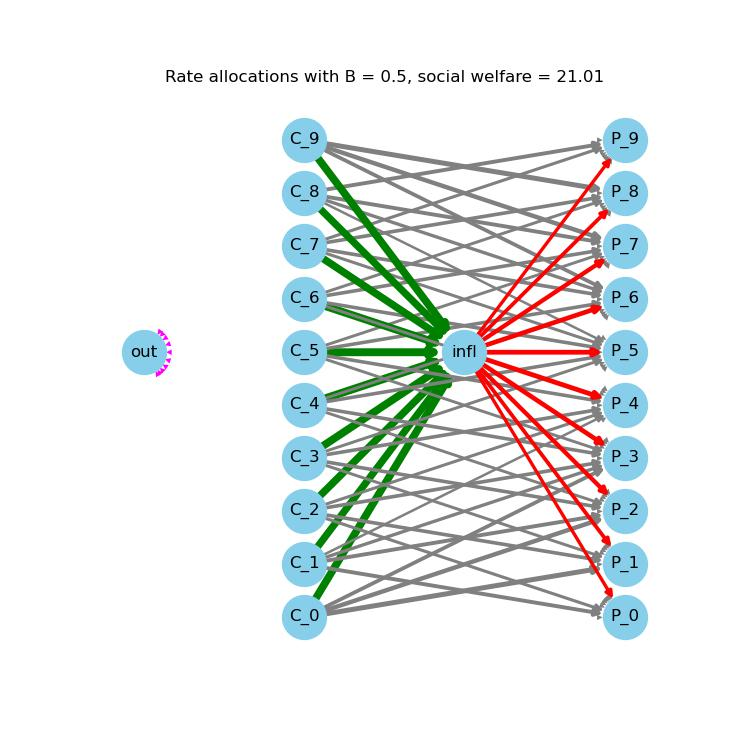
\includegraphics[width=\linewidth]{figures/B_0/0.5_allocs.jpg}
    \end{subfigure}
    \begin{subfigure}[b]{0.45\textwidth}
      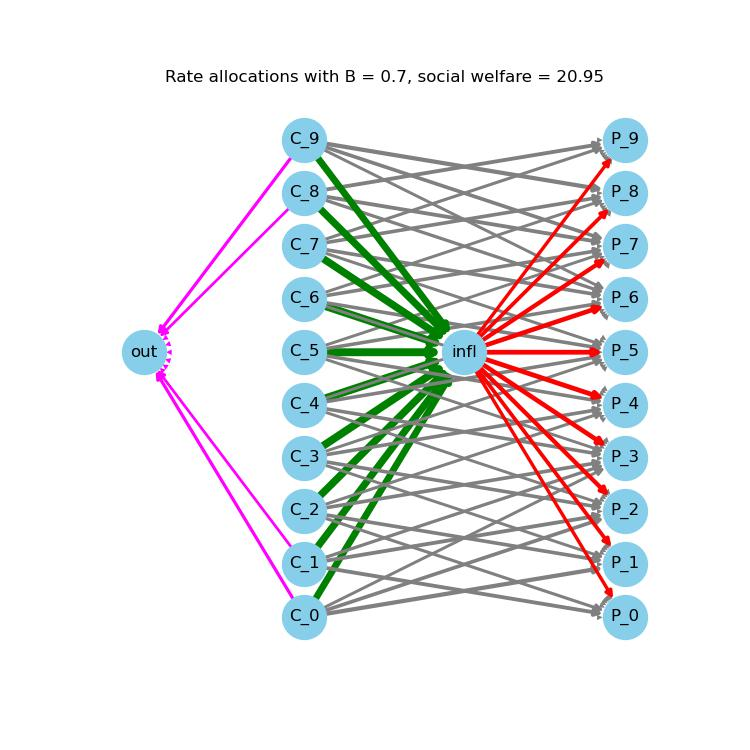
\includegraphics[width=\linewidth]{figures/B_0/0.7_allocs.jpg}
    \end{subfigure}
    \begin{subfigure}[b]{0.45\textwidth}
        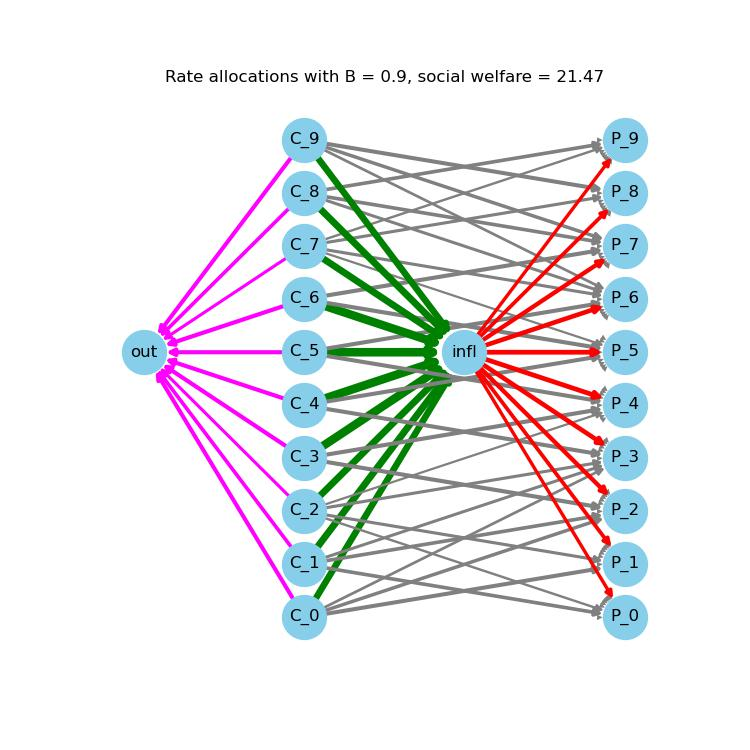
\includegraphics[width=\linewidth]{figures/B_0/0.9_allocs.jpg}
    \end{subfigure}
\end{adjustbox}
\caption{Rate allocations for different outside source interest probabilities}
\label{fig:B_0}
\end{figure}

\Cref{fig:B_0} represents the resulting rate allocation for different values of the parameter \(B_0\), which represents the probability that a content item created by an outside source is of interest to a consumer.

As the consumers become more likely to be interested in outside content, the rate of following from the consumers to outside sources also increase, as expected. This also leads to less following to content producers, because the consumers' total following budget remains fixed. Note that the influencer following remains more-or-less unaffected.

\subsection{Consumer interest function}

The function that a consumer with main interest \(y\) would be interested in a content topic \(x\) is given by \(f(|x-y|)\). As mentioned previously, this function is assumed to be decreasing, because content topics that are further away are of less interest to the consumer.

We consider three different cases for this function:
\begin{itemize}
    \item The function descends rapidly (\(f(x) = e^{-4x}\)): consumers very quickly lose interest in topics as the topic strays from the consumer's main interest.
    \item The function descends linearly (\(f(x) = 1 - 0.5x\)): the neutral case, in which consumers lose interest at a rate proportional to its distance from their main interest.
    \item The function descends slowly (\(f(x) = 1 + e^{-8} - e^{4 x - 8}\)): consumers still retain more of their interest in topics, as the topic strays from the consumer's main interest.
\end{itemize}

\begin{figure}[h]
    \begin{adjustbox}{max width=1.5\textwidth,center}
        \centering
        \begin{subfigure}[b]{0.4\textwidth}
          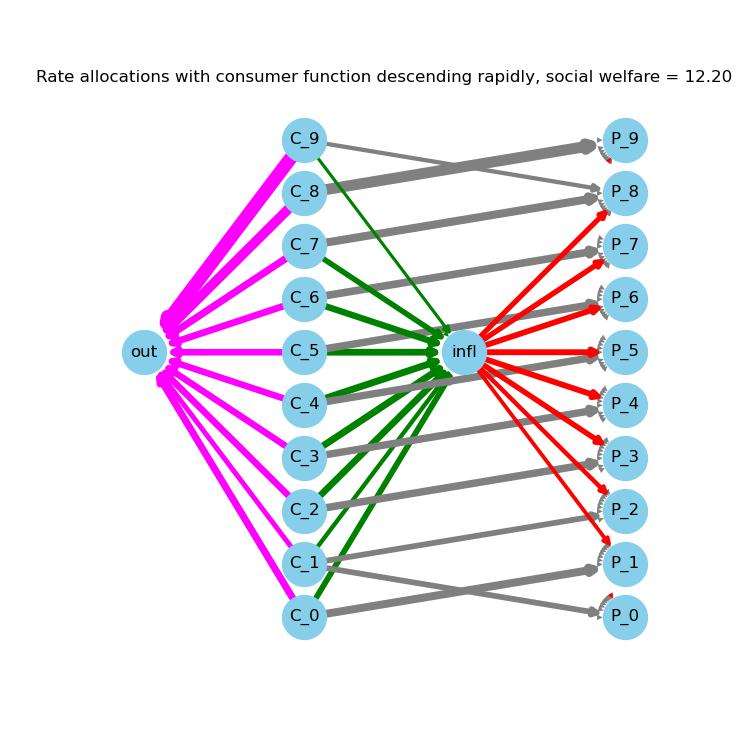
\includegraphics[width=\linewidth]{"figures/f/descending rapidly_allocs.jpg"}
        \end{subfigure}
        \begin{subfigure}[b]{0.4\textwidth}
          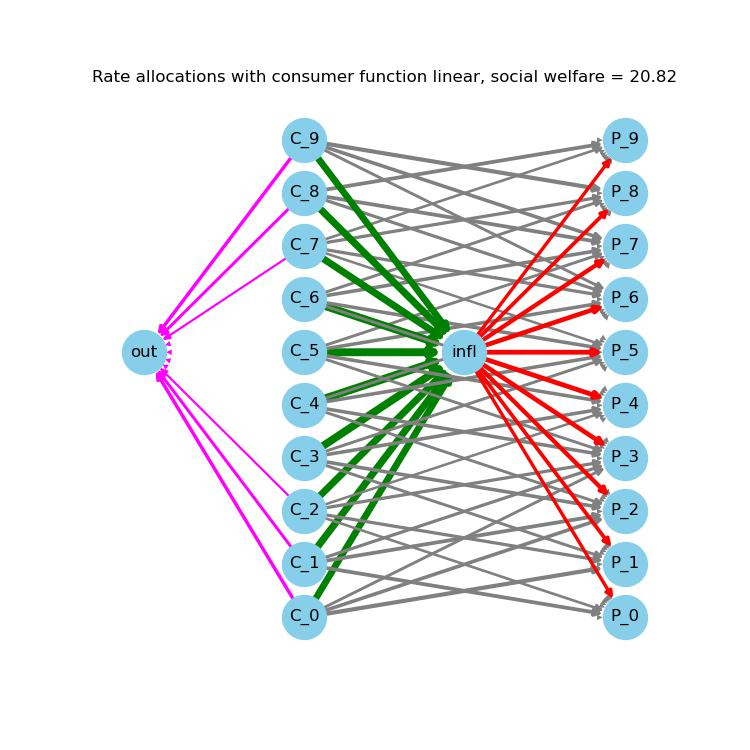
\includegraphics[width=\linewidth]{"figures/f/linear_allocs.jpg"}
        \end{subfigure}
        \begin{subfigure}[b]{0.4\textwidth}
            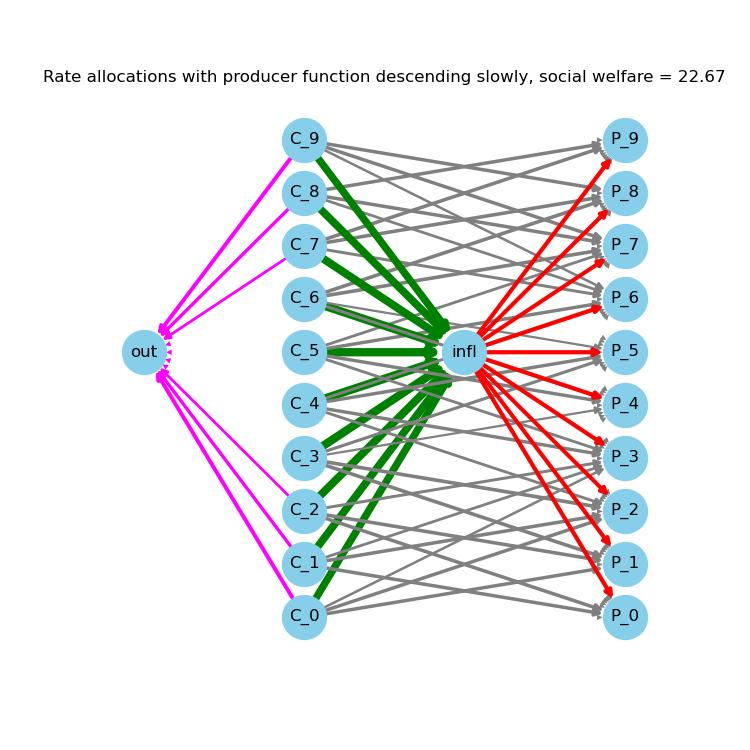
\includegraphics[width=\linewidth]{"figures/f/descending slowly_allocs.jpg"}
        \end{subfigure}
    \end{adjustbox}
\caption{Rate allocations for different consumer interest functions: descending rapidly, linear, and descending slowly}
\label{fig:f}
\end{figure}

\Cref{fig:f} represents these three different cases. If the consumer loses interest quickly, then most of their attention is given to outside sources, with very little to the influencer. Most of the consumers only follow a single producer. As the consumer starts retaining more interest in the linear and descending slowly cases, they progressively give less of their attention to outside sources and more to the influencer and producers. The social welfare also increases. This implies that when the consumers are more interested in the topics in a community as a whole, they are more inclined to follow content sources within a community and gain more benefit from it.

\subsection{Producer interest function}

The ability of a producer with main interest \(y\) to produce content in content topic \(x\) is given by \(g(|x-y|)\); similarly to above, this is also assumed to be decreasing. We can then model different possibilities of \(g\), using the same functions representing the cases of descending rapidly, linear, and descending slowly as above. 

\begin{figure}[h]
\centering
\begin{subfigure}[b]{0.7\textwidth}
    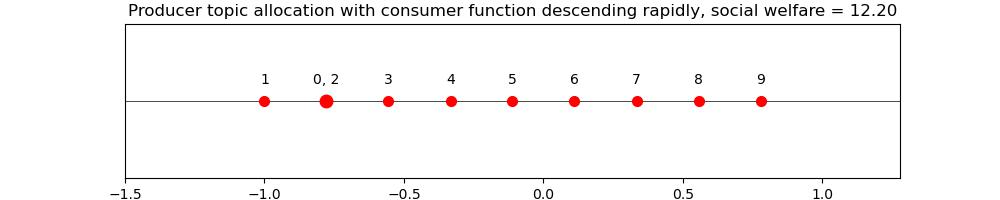
\includegraphics[width=\linewidth]{"figures/g/descending rapidly_topics.jpg"}
\end{subfigure}
\begin{subfigure}[b]{0.7\textwidth}
    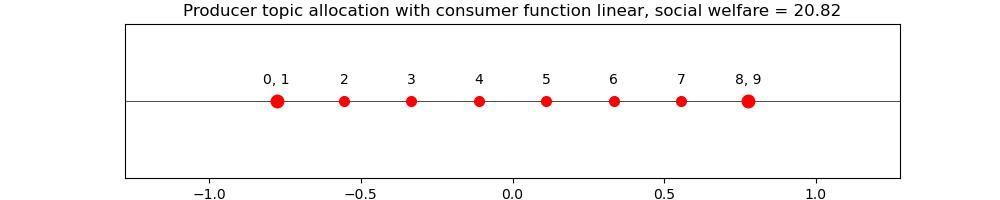
\includegraphics[width=\linewidth]{"figures/g/linear_topics.jpg"}
\end{subfigure}
\begin{subfigure}[b]{0.7\textwidth}
    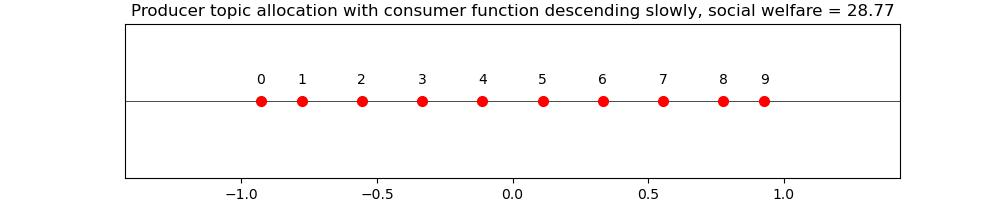
\includegraphics[width=\linewidth]{"figures/g/descending slowly_topics.jpg"}
\end{subfigure}
\caption{Rate allocations for different producer interest functions: descending rapidly, linear, and descending slowly}
\label{fig:g}
\end{figure}

\Cref{fig:g} represents the resulting patterns in the producer topics allocations. The obvious trend emerges: when producers are not as able to produce topics beyond their main interest (i.e. \(g\) descends rapidly), they tend to produce topics closer to their main interests. However, when producers are more able to produce a variety of topics (\(g\) descends more slowly), then their topic of content production strays further from their main interests. In fact, clusters are formed based on multiple producers choosing the same topic, implying that the producers are finding optimal topics to produce content on.

Note that there is minimal difference in the social welfare within the three cases.

\subsection{Rate budgets}

The rate budgets represent the maximum amount of attention that the influencer and each consumer can allocate to the sources they share or consume. 

\begin{figure}[h]
    \centering
\begin{adjustbox}{max width=1.5\textwidth,center}
    \begin{subfigure}[b]{0.4\textwidth}
        \includegraphics[width=\linewidth]{"figures/M_INFL/1.0_allocs.jpg"}
    \end{subfigure}
    \begin{subfigure}[b]{0.4\textwidth}
        \includegraphics[width=\linewidth]{"figures/M_INFL/5.0_allocs.jpg"}
    \end{subfigure}
    \begin{subfigure}[b]{0.4\textwidth}
        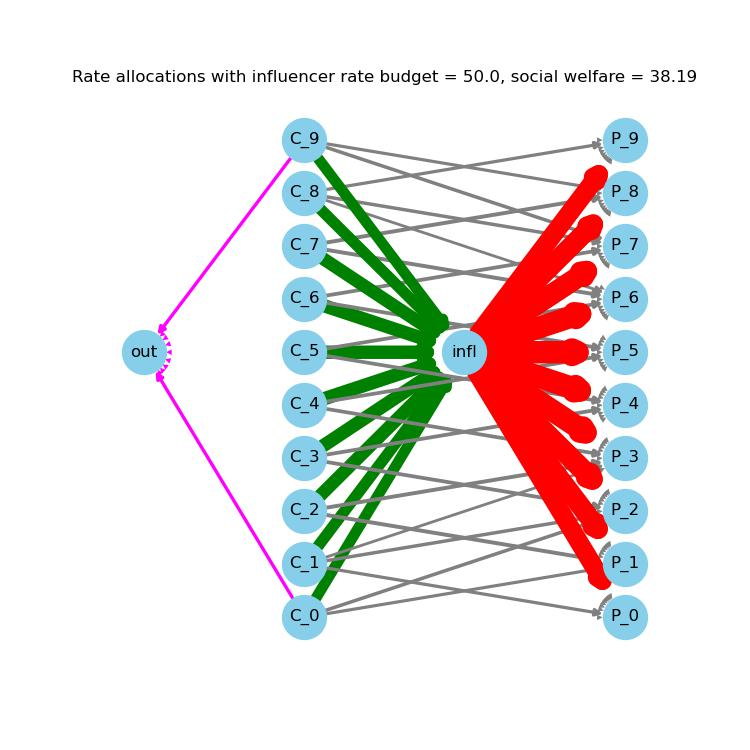
\includegraphics[width=\linewidth]{"figures/M_INFL/50.0_allocs.jpg"}
    \end{subfigure}
\end{adjustbox}
\caption{Different influencer rate budgets, where consumer rate budget = 5.0}
\label{fig:M_INFL}
\end{figure}

\Cref{fig:M_INFL} shows the resulting allocations when the influencer rate budget is changed. Unsurprisingly, as the influencer budget increases, the influencer is able to distribute its attention to more producers and at a higher amount. The consumers also devote more of their allocation to the influencer and less to producers and outside sources, as the influencer rate budget increases. Thus, the influencer plays a greater role in providing value to consumers when it has more attention to give to the community.

\begin{figure}[h]
\centering
\begin{adjustbox}{max width=1.5\textwidth,center}
    \begin{subfigure}[b]{0.4\textwidth}
        \includegraphics[width=\linewidth]{"figures/M/1.0_allocs.jpg"}
    \end{subfigure}
    \begin{subfigure}[b]{0.4\textwidth}
        \includegraphics[width=\linewidth]{"figures/M/5.0_allocs.jpg"}
    \end{subfigure}
    \begin{subfigure}[b]{0.4\textwidth}
        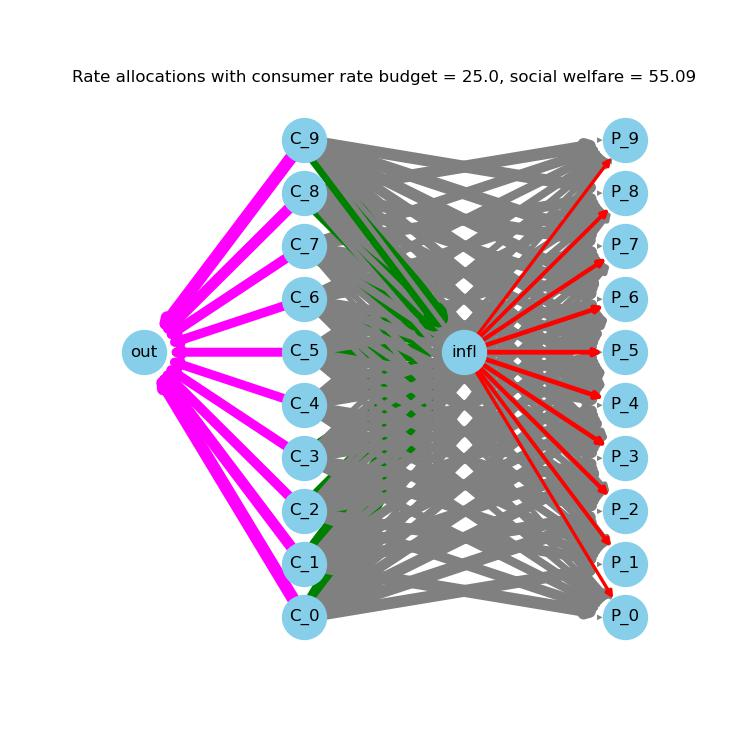
\includegraphics[width=\linewidth]{"figures/M/25.0_allocs.jpg"}
    \end{subfigure}
\end{adjustbox}
\caption{Different consumer rate budgets, where influencer rate budget = 10.0}
\label{fig:M}
\end{figure}

\Cref{fig:M} shows the resulting allocations for different values of the consumer rate budget. The results are perhaps unsurprising; when the consumer rate budget increases, it follows more sources (including the influencer and outside sources) at a greater rate. Note that when the consumer rate budget is low, the consumers use that very limited budget to follow the influencer and not any other sources, again confirming the influencer's importance in providing value to the community.

Note that when either rate budget is increased, the social welfare of the community increases along with it, as expected.

\subsection{Limited information}

In the limited information case, the producers no longer have access to the consumer's choices and must make decisions to optimize for the influencer's attention. To analyze this case effectively and exaggerate its effects, we make some changes from the default parameters. We decrease the influencer rate budget from 10.0 to 5.0, and we set the producer interest function to decrease slowly, meaning that producers would be more flexible in the topics they produce content on.

\begin{figure}[h]
    \centering
        \begin{subfigure}[b]{0.7\textwidth}
            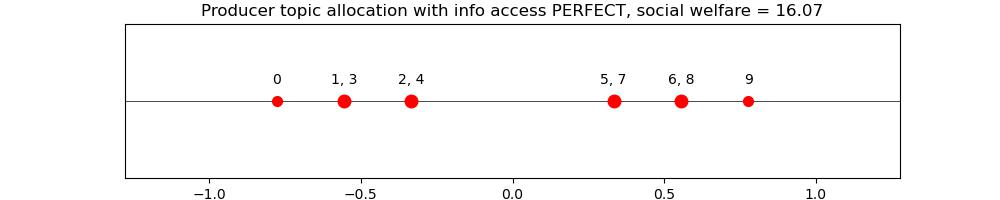
\includegraphics[width=\linewidth]{"figures/lim/1_topics.jpg"}
        \end{subfigure}
        \begin{subfigure}[b]{0.7\textwidth}
            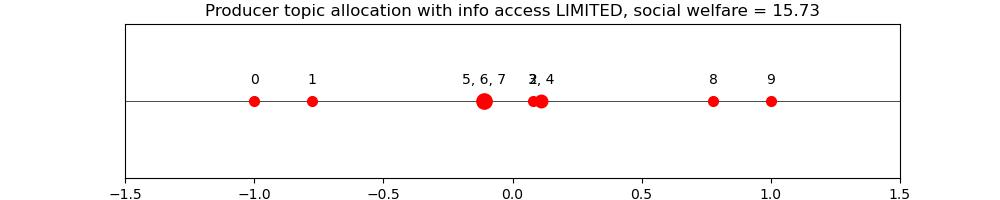
\includegraphics[width=\linewidth]{"figures/lim/2_topics.jpg"}
        \end{subfigure}
\caption{Producer topic allocation for perfect and limited information}
\label{fig:lim_topics}
\end{figure}

\Cref{fig:lim_topics} displays the resulting producer topic allocations for the perfect and limited information cases. The trend of topics clustering towards the average is relatively even in the perfect information case. However, for the limited information case, the producers with main interests close to the average tend to strongly cluster their topics together around that average, whereas the producers further away from the average ignore this clustering effect.

\begin{figure}[h]
    \centering
    \begin{adjustbox}{max width=1.5\textwidth,center}
        \begin{subfigure}[b]{0.6\textwidth}
            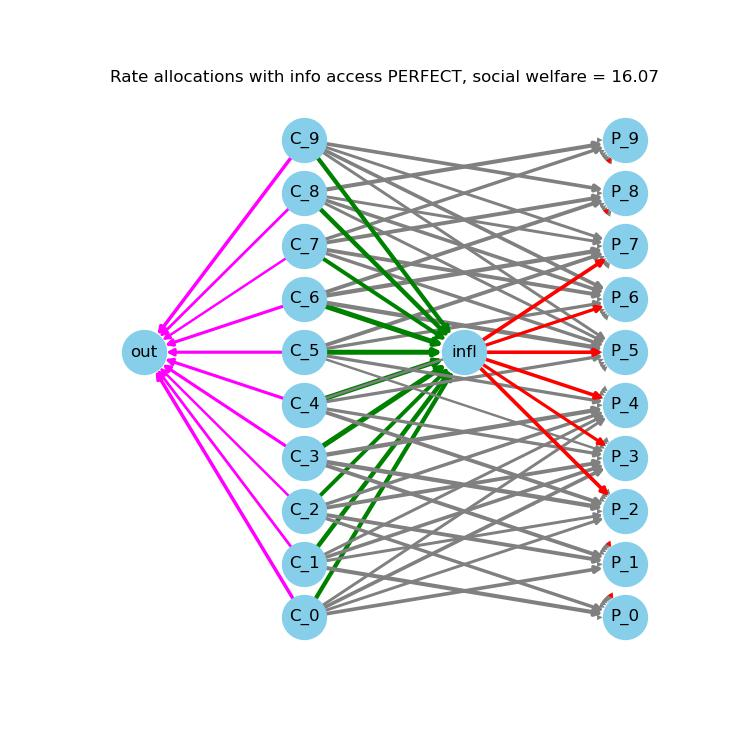
\includegraphics[width=\linewidth]{"figures/lim/1_allocs.jpg"}
        \end{subfigure}
        \begin{subfigure}[b]{0.6\textwidth}
            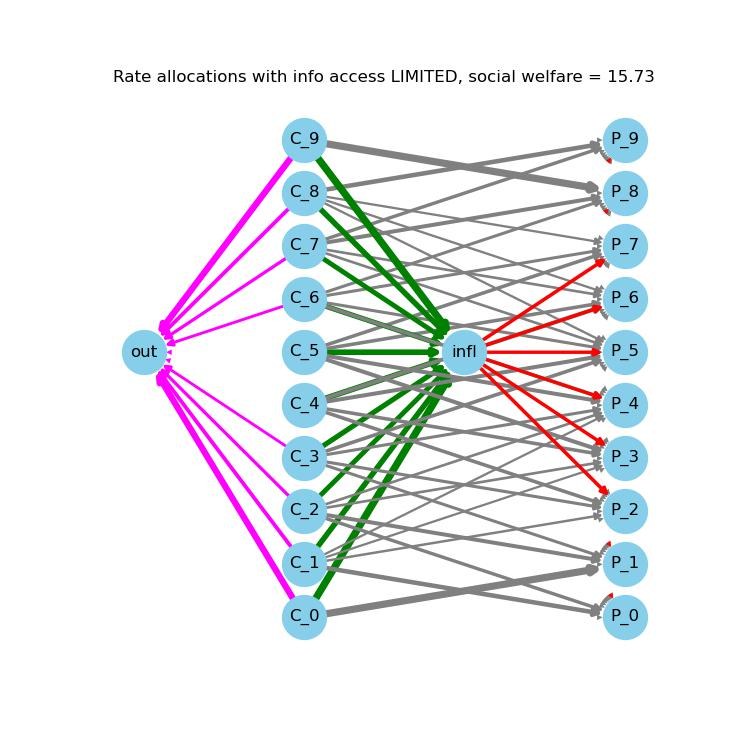
\includegraphics[width=\linewidth]{"figures/lim/2_allocs.jpg"}
        \end{subfigure}
    \end{adjustbox}
\caption{Rate allocations for perfect and limited information}
\label{fig:lim_allocs}
\end{figure}

A similar pattern of differing behaviour due to proximity from the average is shown in \cref{fig:lim_allocs}, which displays the resulting rate allocations in the perfect and limited information case. Overall when comparing the limited information allocation to the perfect information allocation, more attention is given by all consumers to the influencer. However, the consumers with main interests closer to the average divert more attention to the producers, while the consumers with main interest away from the average put more emphasis on outside sources, away from producers. 

\begin{figure}[h]
    \centering
    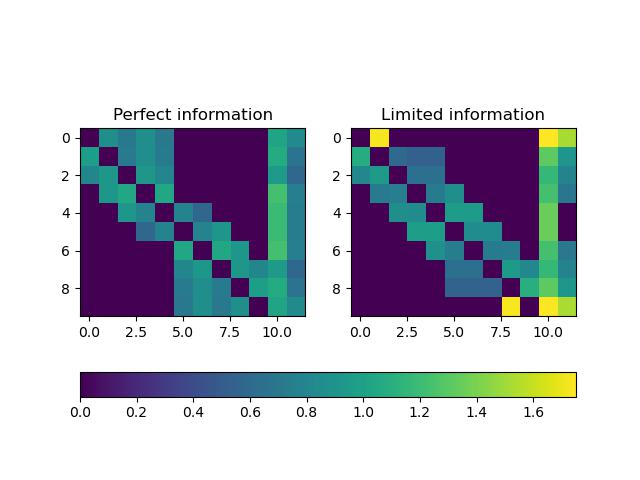
\includegraphics[width=0.7\textwidth]{"figures/lim/colormap.jpg"}
\caption{Consumer allocation colormap for perfect and limited information: row \(i\), column \(j\) represents how much consumer \(i\) allocates to producer \(j\), except for the rightmost column (outside sources) and the column second to the right (influencer).}
\label{fig:lim_allocs_colormap}
\end{figure}

\Cref{fig:lim_allocs_colormap} displays this same consumer rate allocation as a colormap. The same trends can be seen in a different way. For limited information, more attention is being placed to the influencer (the lighter colours on the column second to the right). However, there is differing behaviours depending on how close the consumer is to the average (how close the row is to the middle). The consumers in the middle rows increase their following to producers (increasing the blue/green squares in the middle) and decrease their following to outside sources (the dark squares in the rightmost column). However, the consumers in the top and bottom rows decrease their following to producers (darkening most squares) while increasing their following to outside sources and the influencer (the rightmost two columns).

Therefore, the limited information case increases the community engagement of those with main interests close to the community average; however, it decreases the community engagement of those further away from the average. In essence, shifting the producer's focus from optimizing for the community to optimizing for the influencer creates a hierarchy within the community: those who are already served well by the community are able to extract even more value from it, whereas the ones with more fringe interests are forced to look elsewhere.

\pagebreak

\section{Comparison with empirical results}

The paper \textit{Final Report} applies this content market model to a real-life Twitter community, using Twitter data. It takes a community--a specific set of users--and considers the tweets made by members within this community as the content within the content market. The social support is indicated by the number of retweets for the different tweets.

For our analysis, we will focus on the empirical results given in that paper for community 4 (as listed in the paper), which is a community centred around the topic of machine learning. The paper creates a content market model using the 59123 tweets produced by this 196-member community within the months of June 2020 and April 2023 (inclusive). 

Note that the empirical model assumes the existence of multiple influencers within a community, which differs from the single-influencer assumption of our model.

Our goal is to find the parameters of our model that will most closely align with the empirical model. To do, we investigate two different plots given by

\subsection{Consumer allocations}

\begin{figure}[h]
    \centering
    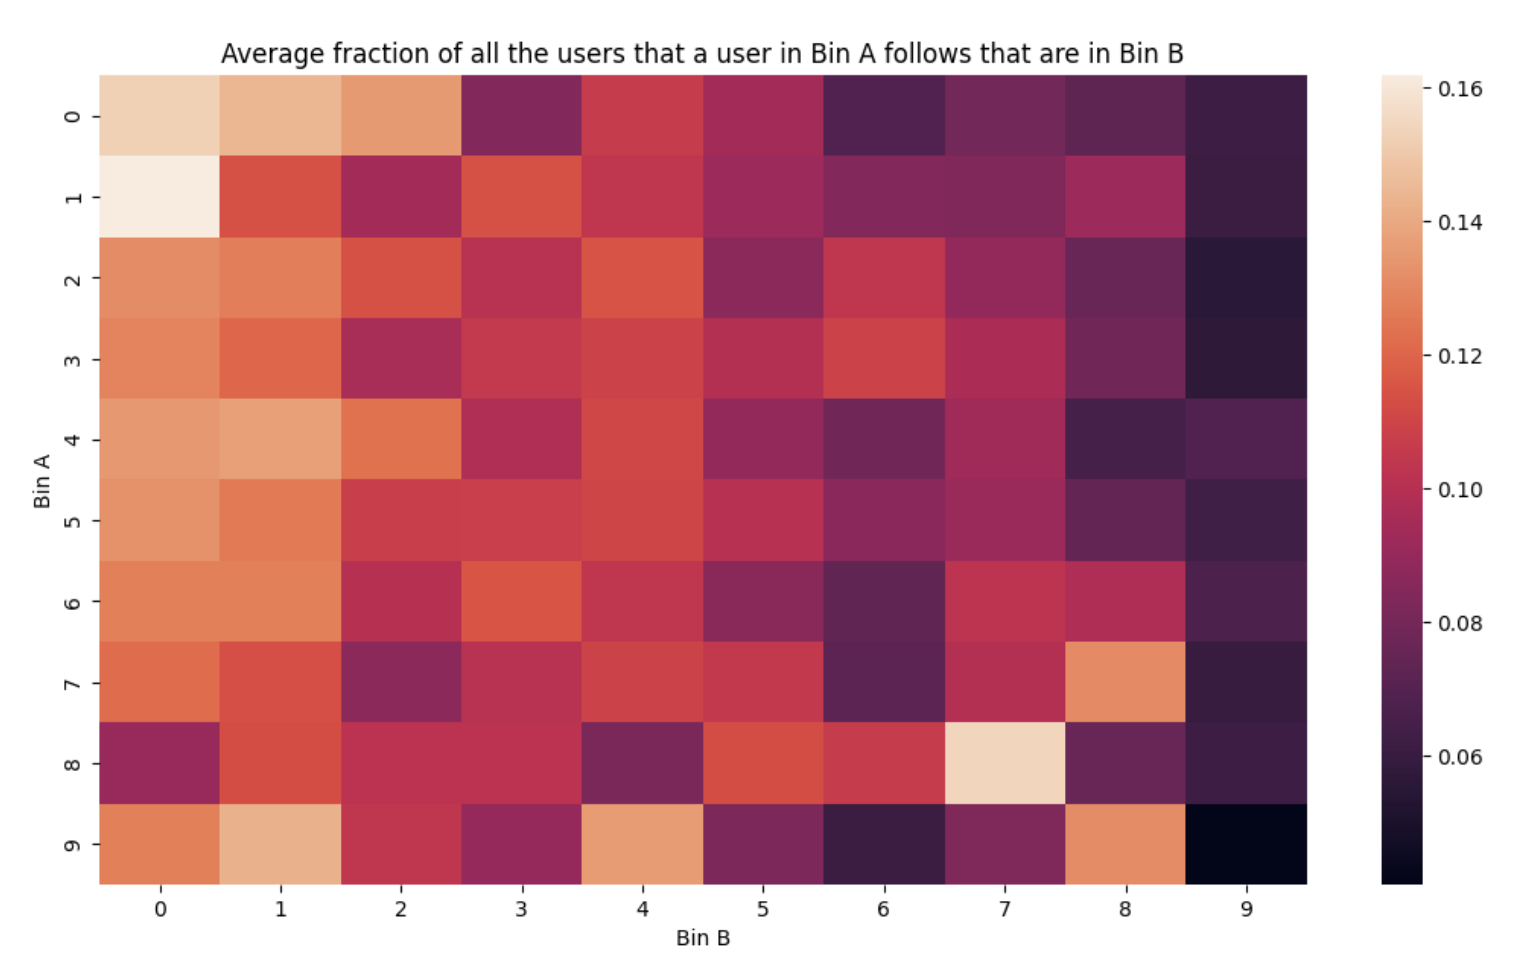
\includegraphics[width=0.7\textwidth]{figures/rachel_heatmap.png}
    \caption{The empirical consumer allocations}
    \label{fig:rachel_heatmap}
\end{figure}

\Cref{fig:rachel_heatmap} displays the empirical consumer allocations as a heatmap, as given within \textit{Final Report}. Note that it differs from the consumer allocations we have shown previously in our paper (for example in \cref{fig:lim_allocs_colormap}). Because there are many more than 10 users, it bins the users using their social support rank. This means that bin 0 aggregates data for the users with the top social supports, bin 1 aggregates data for the users with the next highest social supports, and so on. Outside sources are ignored. Each block at row \(i\) and column \(j\) therefore represents the rate at which consumers in bin \(i\) follow producers in bin \(j\). Furthermore, the influencers are set to be bin 0, meaning that they are treated just to be the users with the highest social support.

We also display our data in a similar way. While we still use individual users instead of bins, we order our columns based on how close their main interests are to the average; this way, the consumer represented by the first column has the closest main interest to the average main interest, the consumer represented by the second column is the second closest, and so on. The same is done for the producers. As discussed previously, members with main interests closer to the average have more social support and devote more attention to the community, so this ordering matches with the ordering of users in the empirical heatmap.

We also set our model to have 9 members and 1 influencer (to match with the 10 bins in \cref{fig:rachel_heatmap}), and to have the influencer and consumer rate budget both be \(5.0\). We will experiment with different values later on. 

\subsubsection{Consumer interest functions}

\begin{figure}[h]
    \centering
\begin{adjustbox}{max width=1.5\textwidth,center}
    \begin{subfigure}[b]{0.45\textwidth}
        \includegraphics[width=\linewidth]{"figures/f/descending rapidly_heatmap.jpg"}
    \end{subfigure}
    \begin{subfigure}[b]{0.45\textwidth}
        \includegraphics[width=\linewidth]{"figures/f/linear_heatmap.jpg"}
    \end{subfigure}
    \begin{subfigure}[b]{0.45\textwidth}
        \includegraphics[width=\linewidth]{"figures/f/descending slowly_heatmap.jpg"}
    \end{subfigure}
\end{adjustbox}
\caption{Consumer allocations with different consumer interest functions}
\label{fig:f_heatmap}
\end{figure}

\Cref{fig:f_heatmap} represents the consumer allocations with different functions of consumer interest within the community. Note that the sim value represents the cosine similarity between the consumer allocations within our model and the empirical model; a higher cosine similarity indicates our model being closer to the empirical model.

It is obvious that the more slowly the consumer interest function descends (i.e. the more a consumer is interested in topics outside of their main interest), the closer our model gets to the empirical model, both visually as well as numerically. Therefore, we can conclude that in the empirical model, users are interested in consuming content in a great variety of topics, not just their main interest. We can also set the consumer interest functions to be the one that descends slowly in the following analysis.

\subsubsection{Producer interest functions}

\begin{figure}[h]
    \centering
\begin{adjustbox}{max width=1.5\textwidth,center}
    \begin{subfigure}[b]{0.45\textwidth}
        \includegraphics[width=\linewidth]{"figures/g/descending rapidly_heatmap.jpg"}
    \end{subfigure}
    \begin{subfigure}[b]{0.45\textwidth}
        \includegraphics[width=\linewidth]{"figures/g/linear_heatmap.jpg"}
    \end{subfigure}
    \begin{subfigure}[b]{0.45\textwidth}
        \includegraphics[width=\linewidth]{"figures/g/descending slowly_heatmap.jpg"}
    \end{subfigure}
\end{adjustbox}
\caption{Consumer allocations with different producer interest functions}
\label{fig:g_heatmap}
\end{figure}

\Cref{fig:g_heatmap} represents the consumer allocations with different functions for the ability of a producer to produce topics outside of their main interest. It is clear that the producer function does not significantly impact how close the model is to the empirical model; the similarity remains the same, and visually the differences are not very obvious. We could perhaps say that the model where the producer function descends slowly is the closest to empirical, because it displays the strongest trend of colors darkening from left to right, which represents how the consumers closest to the main interest allocate more attention to the community than the consumers further away from the main interest. However, this trend is not strong.

\subsubsection{Influencer rate budgets}\label{sss:M_INFL}

\begin{figure}[h]
    \centering
\begin{adjustbox}{max width=1.5\textwidth,center}
    \begin{subfigure}[b]{0.45\textwidth}
        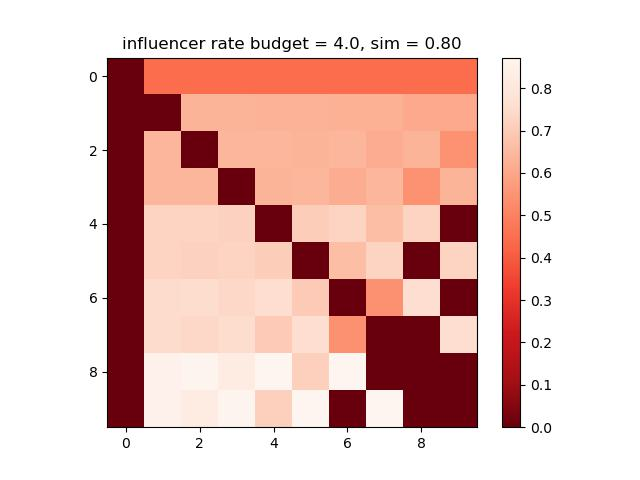
\includegraphics[width=\linewidth]{"figures/M_INFL/4.0_heatmap.jpg"}
    \end{subfigure}
    \begin{subfigure}[b]{0.45\textwidth}
        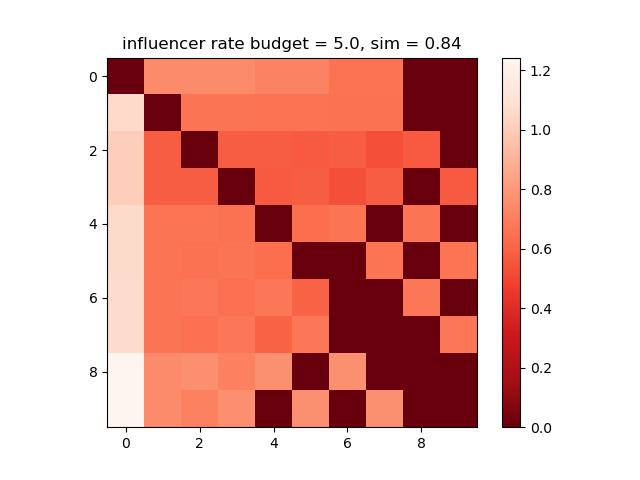
\includegraphics[width=\linewidth]{"figures/M_INFL/5.0_heatmap.jpg"}
    \end{subfigure}
    \begin{subfigure}[b]{0.45\textwidth}
        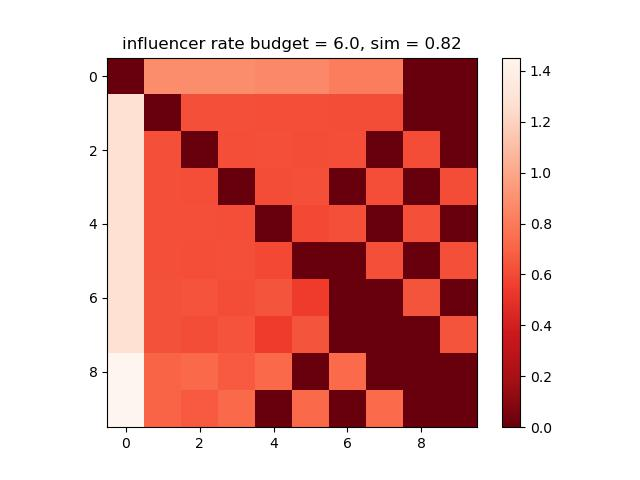
\includegraphics[width=\linewidth]{"figures/M_INFL/6.0_heatmap.jpg"}
    \end{subfigure}
\end{adjustbox}
\caption{Different influencer rate budgets, where consumer rate budget = 5.0}
\label{fig:M_INFL_heatmap}
\end{figure}

\Cref{fig:g_heatmap} represents the consumer allocations with different influencer rate budgets. Based on the cosine similarities as well as the visual appearance of the heatmaps, the case in which the influencer and consumer rate budgets are both equal to \(5.0\) is the closest to the empirical model. This suggests that in the empirical model, all users have the same amount of total attention to allocate to the community, including the influencer. 

\subsubsection{Perfect and limited information}

\begin{figure}[h]
    \centering
\begin{adjustbox}{max width=1.5\textwidth,center}
    \begin{subfigure}[b]{0.45\textwidth}
        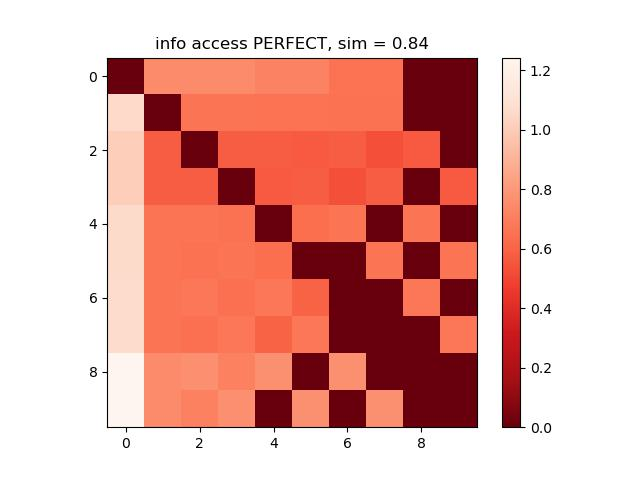
\includegraphics[width=\linewidth]{"figures/lim/1_heatmap.jpg"}
    \end{subfigure}
    \begin{subfigure}[b]{0.45\textwidth}
        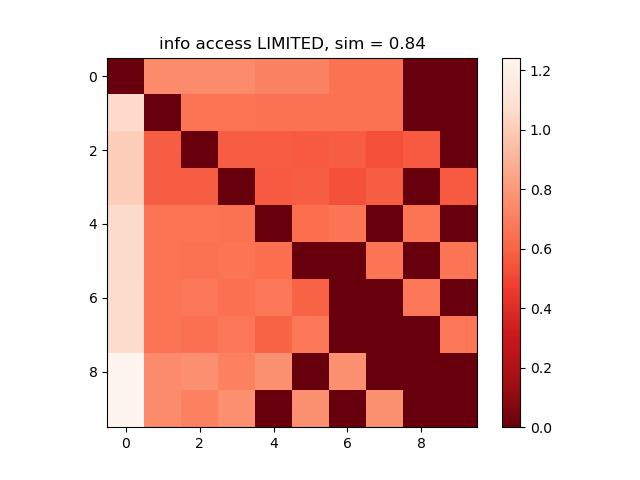
\includegraphics[width=\linewidth]{"figures/lim/2_heatmap.jpg"}
    \end{subfigure}
\end{adjustbox}
\caption{Consumer allocations for perfect vs. limited information}
\label{fig:lim_heatmap}
\end{figure}

For our research, we also tested the cases the producers have perfect access to all the information about consumer social support, as well as when they only have limited information on the influencer's social support. \Cref{fig:lim_heatmap} shows that this makes no difference to the consumer allocations. Note that this may seem to contradict with \cref{fig:lim_allocs_colormap}, which did show a difference in allocations between the perfect and limited information case; however, \cref{fig:lim_allocs_colormap} visualized a model with parameters especially chosen to exaggerate the differences between the perfect and limited information cases, which is different from the parameters of our model.

\subsection{Social Support}

\begin{figure}[h]
    \centering
    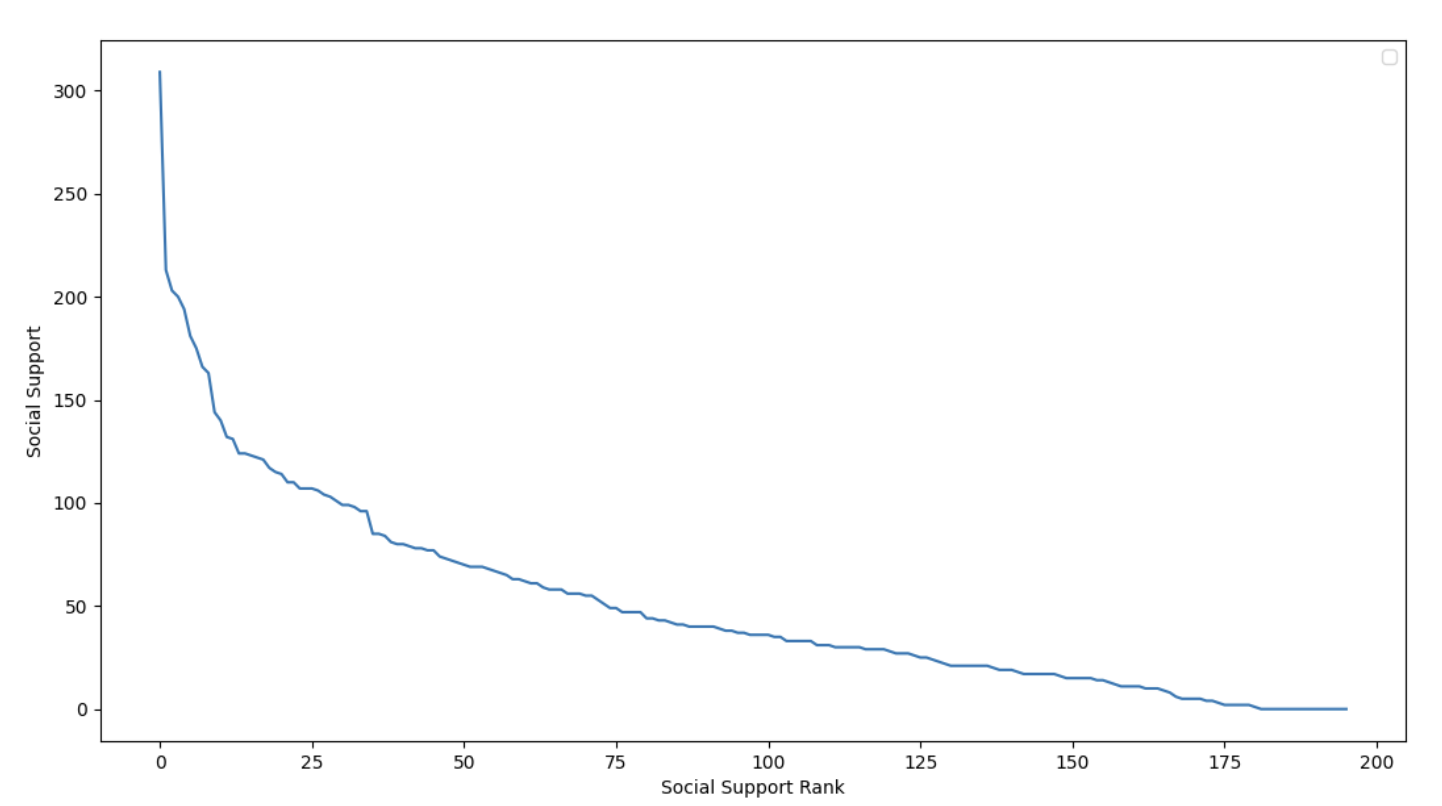
\includegraphics[width=0.7\textwidth]{figures/rachel_supps.png}
    \caption{The empirical social supports in descending order}
    \label{fig:rachel_supps}
\end{figure}

Another set of graphs analyzed within \textit{Final Report} are the graphs of social support in a community, graphed in descending order. This is shown in \cref{fig:rachel_supps}, and there is a clear negative exponential trend for how the social supports decrease. Essentially, a small number of users have lots of social support, whereas most users have minimal social support.

Because of computational constraints and because we are only trying to analyze the general trend, our model will only have 26 agents (25 members and 1 influencer), instead of the 196 within the empirical model. We again set the default influencer and consumer rate budgets to be 5.0, supported by the investigation of \cref{sss:M_INFL}.

\subsubsection{Consumer interest functions}

\begin{figure}[h]
    \centering
\begin{adjustbox}{max width=1.5\textwidth,center}
    \begin{subfigure}[b]{0.45\textwidth}
        \includegraphics[width=\linewidth]{"figures/f/descending rapidly_supps.jpg"}
    \end{subfigure}
    \begin{subfigure}[b]{0.45\textwidth}
        \includegraphics[width=\linewidth]{"figures/f/linear_supps.jpg"}
    \end{subfigure}
    \begin{subfigure}[b]{0.45\textwidth}
        \includegraphics[width=\linewidth]{"figures/f/descending slowly_supps.jpg"}
    \end{subfigure}
\end{adjustbox}
\caption{Social supports with different consumer interest functions}
\label{fig:f_supps}
\end{figure}

\Cref{fig:f_supps} shows the social supports within our model in descending order. Clearly, the negative exponential trend is not there; most users have relatively high social support, and a small number of users have little to no social support. However, in the case where the consumer interest function decreases slowly, the trend does seem to decrease in a more linear fashion, which is closer to the empirical model. Therefore, we can conclude that in the empirical model, consumers are generally still relatively interested in topics outside their main interest; this agrees with our earlier investigation using the consumer allocation heatmaps. 

\subsubsection{Producer interest functions}

\begin{figure}[h]
    \centering
\begin{adjustbox}{max width=1.5\textwidth,center}
    \begin{subfigure}[b]{0.45\textwidth}
        \includegraphics[width=\linewidth]{"figures/g/descending rapidly_supps.jpg"}
    \end{subfigure}
    \begin{subfigure}[b]{0.45\textwidth}
        \includegraphics[width=\linewidth]{"figures/g/linear_supps.jpg"}
    \end{subfigure}
    \begin{subfigure}[b]{0.45\textwidth}
        \includegraphics[width=\linewidth]{"figures/g/descending slowly_supps.jpg"}
    \end{subfigure}
\end{adjustbox}
\caption{Social supports with different producer interest functions}
\label{fig:g_supps}
\end{figure}

\Cref{fig:g_supps} shows the the social support graphs with different producer interest functions. We see again that the differences are very small, and that the producer interest function does not play a major role in whether our model is a good approximation of the empirical model, from the perspective of social supports.

\subsubsection{Influencer rate allocations}

\begin{figure}[h]
    \centering
\begin{adjustbox}{max width=1.5\textwidth,center}
    \begin{subfigure}[b]{0.45\textwidth}
        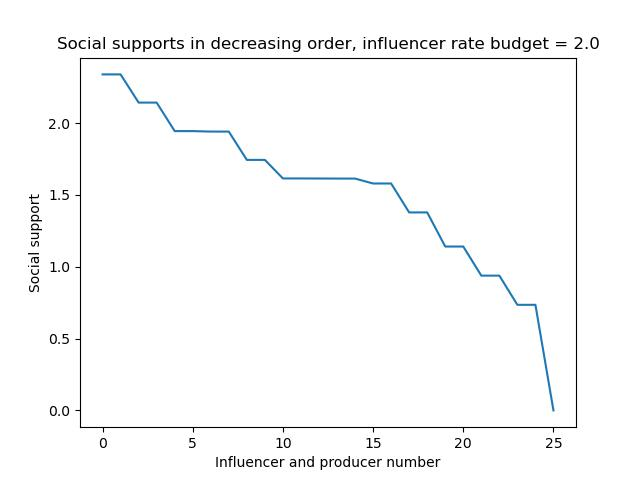
\includegraphics[width=\linewidth]{"figures/M_INFL/2.0_supps.jpg"}
    \end{subfigure}
    \begin{subfigure}[b]{0.45\textwidth}
        \includegraphics[width=\linewidth]{"figures/M_INFL/5.0_supps.jpg"}
    \end{subfigure}
    \begin{subfigure}[b]{0.45\textwidth}
        \includegraphics[width=\linewidth]{"figures/M_INFL/8.0_supps.jpg"}
    \end{subfigure}
\end{adjustbox}
\caption{Social supports with different influencer rate budgets, where consumer rate budget = 5.0}
\label{fig:M_INFL_supps}
\end{figure}

\Cref{fig:M_INFL_supps} shows the social supports for different influencer rate budgets. Upon immediate visual inspection, it is perhaps tempting to say that the case in which the influencer rate budget is high (the rightmost graph) is the closest to the empirical results, since we can observe what seems like a sharp exponential decrease. However, this sharp exponential decrease is just the decrease from influencer to producer social supports; after that, no such decrease is observed, and the negative exponential trend is not found within the rest of the producer social supports.

Therefore, the case where the influencer and consumer rate budgets are equal (the middle graph) can still be taken as the closest case to the empirical values, based on the previous results from the consumer allocation heatmaps.

\subsubsection{Perfect and limited information}

\begin{figure}[h]
    \centering
\begin{adjustbox}{max width=1.5\textwidth,center}
    \begin{subfigure}[b]{0.45\textwidth}
        \includegraphics[width=\linewidth]{"figures/lim/1_supps.jpg"}
    \end{subfigure}
    \begin{subfigure}[b]{0.45\textwidth}
        \includegraphics[width=\linewidth]{"figures/lim/2_supps.jpg"}
    \end{subfigure}
\end{adjustbox}
\caption{Social supports for perfect vs limited information}
\label{fig:lim_supps}
\end{figure}

\Cref{fig:lim_supps} shows the social supports in the case where the producers have perfect information to all consumer social supports, as well as the case where they have limited information to only the influencer's social support. Unlike the consumer allocation heatmaps in which the information access did not play a major role, here we see a big difference; the limited information graph matches the negative exponential trend in the empirical graph significantly more closely than the perfect information graph. Thus, we can conclude that the producers do indeed optimize moreso for the influencer's social support than for all consumers, and the limited information model is a more accurate representation of Twitter as a content market.

\pagebreak

\section{Conclusion}

We discussed the way in which the final consumer attention, influencer attention, and producer topic allocations were affected by various parameters: community size, probability of being interested in outside sources, different functions representing consumer and producer interest, rate budgets, and the producer's access to information. We found patterns in the resulting rate and topic allocations by modifying these parameters, and we explained those patterns using ideas from community behaviour and content engagement.

This model was designed specifically with an online community on social media in mind. However, its core idea---a content network involving those consuming content and giving support to it, those producing content, and those distributing and aggregating it---can be applied to domains far beyond online social networks. An artistic network involves artists who create their art, an audience to view the art, and curators and exhibitors who gather the art and exhibit it to the community. An academic network is composed of researchers who write papers and create results, an audience who is consumes those results for their own gain, and journals and conferences to aggregate and publish the work. A business network involves companies that create a product, a target audience to use the product, and salespeople who market the product to the audience. This goes to show the power of complex network theory; we can apply the same methods of analysis to disparate domains, creating connections in the structural properties of very different networks. 

One interesting way in which this model differs from many existing models of social media is its distinction between those who produce the content, and those who distribute it (the influencer). When thinking of the term "influencer" in the context of social networks, it is tempting to think of a social media influencer who creates content to directly influence their following. However, our model thinks of the conception of an influencer differently. While an influencer may produce content, we consider its power to be in being attuned to the interests of the community as a whole and sharing content to create the most benefit for the community. They influence the content that the community sees, due to the larger following that they receive from the community. This is particularly true of the limited information case, in which the producers are working to get the influencer to share them more, rather than directly increasing the value of their content to the consumers. However, as seen previously, the influencer's increased power in the limited information case leads to potential inequity within the community. Those already closely interested in the content benefit more from the influencer's power, and those who are not as involved will seek outside sources and even potentially leave the community. 

The politics of community members joining and leaving is a potentially interesting area of exploration. Our model assumes a static set of community members that do not join or leave, where the rate of content production for producers remains constant. A more detailed model could allow community members to leave once they feel that outside sources are more beneficial to the community, or to produce less or more content depending on how involved they are in the community. The model could also take into account the potential for new members joining, as well as how these communities form in the first place. This idea is explored in the paper \textit{Core-Periphery Community Formation and the Winner-Take-All Effect}, which provides a mathematical criteria for the formation of a community and the development of a core-periphery structure. We could explore this using our multi-agent model, adding this dynamism to the structure of the model.

Furthermore, our model makes the important assumption that the social support that a consumer gives a content item is proportional to the value the content provides to the consumer. However, this is not necessarily the case; consumers may have reasons of giving social support other than the content providing value, including supporting the producer (ex. liking a friend's post even if the content is not interesting) or increasing visibility to an important subject. Furthermore, different consumers may have patterns of providing social support; some may give social support very liberally, whereas others may be passive and rarely indicate their support. This could be explored by experimenting with different models of social support, and adding individual consumer variation to how it is calculated.

\end{document}